\section{Experimentación General}


\subsection{Comparando con el Exacto}

\quad Debido al costo del exacto se realizaron tests de 3 nodos a 19 con 100 repeticiones para cada cantidad.

\subsubsection{Distancia}

\quad

\quad Comparamos los resultados del algoritmo exacto, el goloso, la búsqueda local y GRASP. Calculamos las distancias a la solución del exacto. 

\quad

\begin{figure}[H]
	\centering
	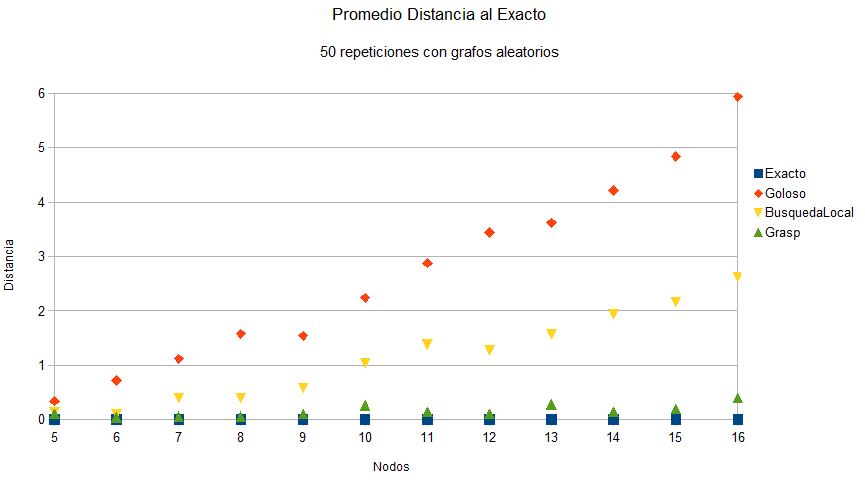
\includegraphics[scale=0.8]{distancia-Azar.png}
\caption{Costos}
\end{figure}

\begin{figure}[H]
	\centering
	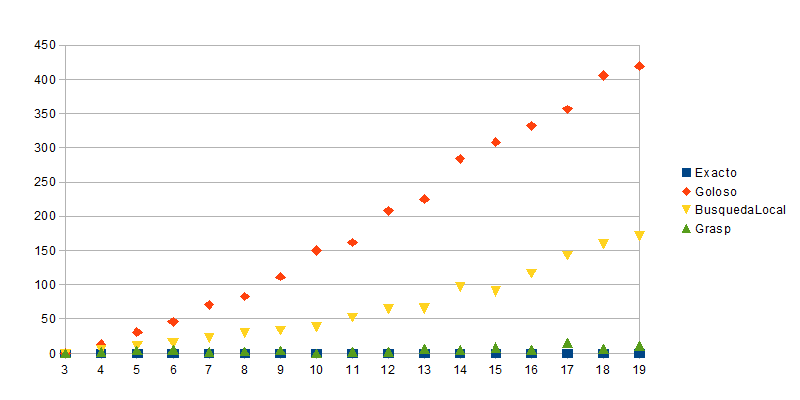
\includegraphics[scale=0.8]{distancia-G-y-H-densos.png}
\caption{Costos}
\end{figure}

\begin{figure}[H]
	\centering
	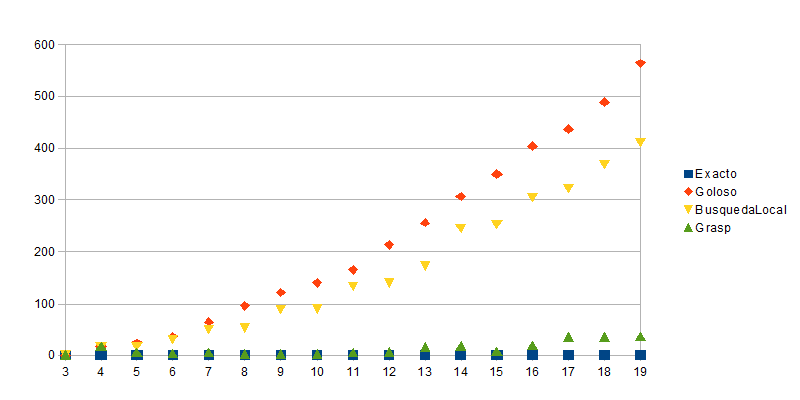
\includegraphics[scale=0.8]{distancia-H-complemento.png}
\caption{Costos}
\end{figure}

\quad

\quad Como se puede observar, casi no hay diferencias entre grafos aleatorios y densos. Aunque con los grafos donde G y H son complementos uno del otro, la búsqueda local aumentó considerablemente su distancia.

\subsubsection{Efectividad}

\quad Ahora consideramos que un resultado es efectivo si dista menos del 10$ % $ del resultado exacto.

\quad

\begin{figure}[H]
	\centering
	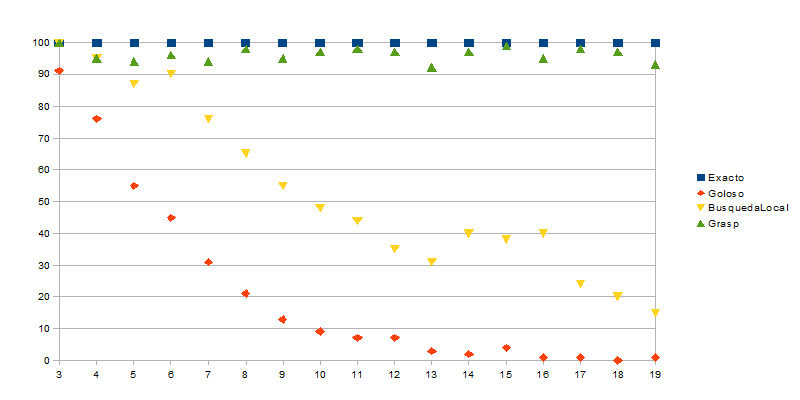
\includegraphics[scale=0.8]{efectividad-Azar.png}
\caption{Costos}
\end{figure}

\begin{figure}[H]
	\centering
	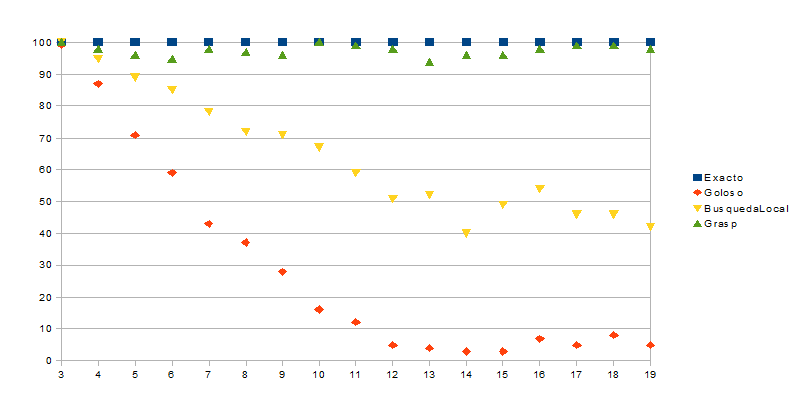
\includegraphics[scale=0.8]{efectividad-G-y-H-densos.png}
\caption{Costos}
\end{figure}

\begin{figure}[H]
	\centering
	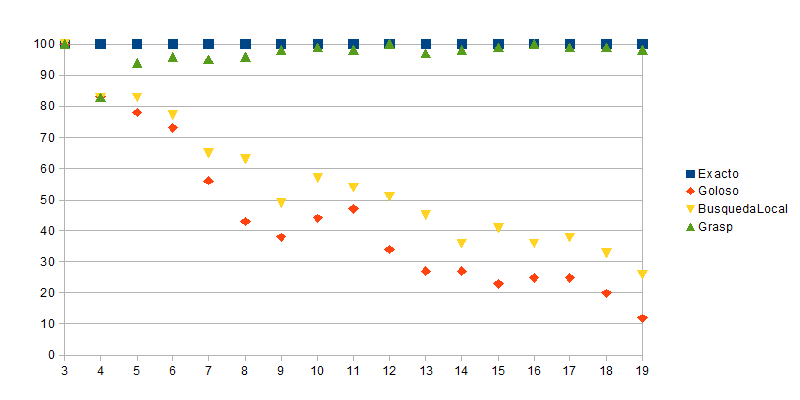
\includegraphics[scale=0.8]{efectividad-H-complemento.png}
\caption{Costos}
\end{figure}

\quad Se observa que para estas cantidades de nodos la efectividad de GRASP no decae, a diferencia de las otras heurísticas.

\subsection{Comparando con Grasp}

\quad Dejando de lado el algoritmo exacto, podemos experimentar con una mayor cantidad de nodos. Comparamos la heuristica golosa, la búsqueda local y GRASP

\subsubsection{Efectividad}

\begin{figure}[H]
	\centering
	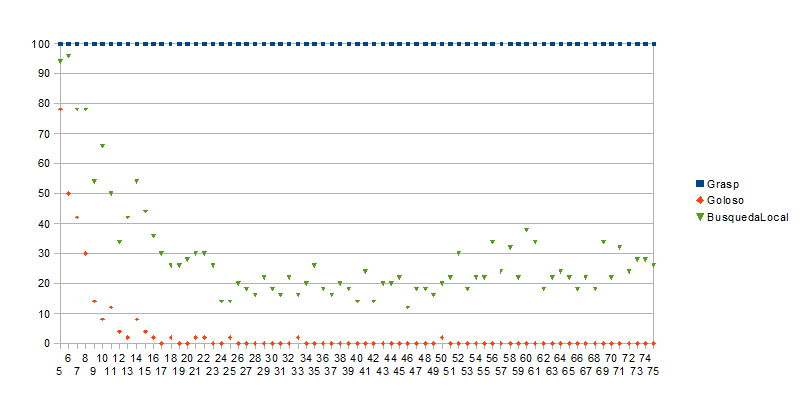
\includegraphics[scale=0.8]{efectividad-vs-grasp.png}
\caption{Costos}
\end{figure}

\quad Podemos ver como a partir de cierto punto, la heurística golosa no es para nada efectiva (según el criterio anteriormente mencionado). En cambio, la búsqueda local se \textit{estanca} entre el 10$ % $ y 40$ % $ de efectividad.

\subsubsection{Costo}

\begin{figure}[H]
	\centering
	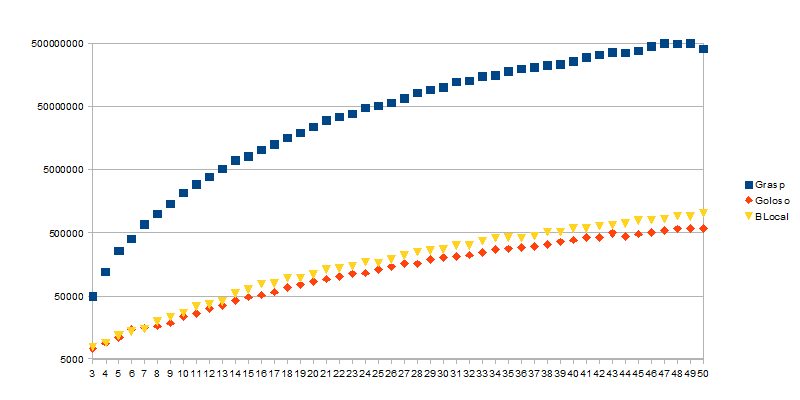
\includegraphics[scale=0.8]{timing-vs-grasp.png}
\caption{Costo temporal de las heurísticas, en escala logaritmica}
\end{figure}

\quad En este gráfico podemos observar como GRASP a pesar de obtener resultados mucho mejores que las otras heuristicas, consume mucho más tiempo de procesamiento.

\quad Si bien la búsqueda local cuesta apenas más que la golosa, en comparación con GRASP, se obtiene muchos mejores resultados.